%% main_ppgco_ufu.tex v1.0, Lásaro Camargos e Denise Guliato
% adaptado de modeloABNT2.tex, v1.0 athila 
% ------------------------------------------------------------------------
% ------------------------------------------------------------------------
% eesc: Modelo de Trabalho Acadêmico (tese de doutorado, dissertação de
% mestrado e trabalhos monográficos em geral) em conformidade com 
% ABNT NBR 14724:2011. Esta classe estende as funcionalidades da classe
% abnTeX2 elaborada de forma a adequar os parâmetros exigidos pelas 
% normas USP e do departamento de elétrica da Escola de Engenharia 
% de São Carlos - USP.
% ------------------------------------------------------------------------
% ------------------------------------------------------------------------

% ------------------------------------------------------------------------
% Opções:
% 	tesedr:     Formata documento para tese de doutorado
%	qualidr:    Formata documento para qualificação de doutorado
% 	dissertmst: Formata documento para dissertação de mestrado
% 	qualimst:   Formata documento para qualificação de mestrado
% ------------------------------------------------------------------------
\documentclass[dissertmst]{ppgco}
%Não altere o comando seguinte. O título de seu trabalho será especificado mais adiante.
\title{Proposta do projeto final de Data Science - Violência Armada e suas tendências futuras nos EUA.  
}

% ---
% PACOTES
% ---

% ---
% Pacotes fundamentais 
% ---
\usepackage{cmap}				% Mapear caracteres especiais no PDF
\usepackage{lmodern}				% Usa a fonte Latin Modern			
\usepackage{makeidx}            	% Cria o indice
\usepackage{hyperref}  			% Controla a formação do índice
\usepackage{lastpage}			% Usado pela Ficha catalográfica
\usepackage{indentfirst}			% Indenta o primeiro parágrafo de cada seção.
\usepackage{nomencl} 			% Lista de simbolos
\usepackage{graphicx}			% Inclusão de gráficos
% ---

% ---
% Pacotes adicionais, usados apenas no âmbito do Modelo eesc
% ---
\usepackage{lipsum}				       % para geração de dummy text
\usepackage[printonlyused]{acronym}
\usepackage[table]{xcolor}
% ---


% ---
% Informações de dados para CAPA e FOLHA DE ROSTO
% ---
%
% Título:
%	1. Título em português
%	2. Título em inglês
\titulo{Proposta do projeto final de Data Science - Violência Armada e suas tendências futuras nos EUA.}{
Proposal of the final Data Science project - Armed Violence and its future trends in the USA}
%
% Autor:
%	1. Nome completo do autor
%	2. Formato de nome para bibliografia
\author{
  Lerisson Florêncio de Freitas\\
  \texttt{lff3@cin.ufpe.br}
  \and\\
  Matheus Raz de Oliveira Leandro\\
  \texttt{mrol@cin.ufpe.br}}
%
% Cidade
\local{Recife}
% Ano de defesa
\data{2018}
%Área de concentração da pesquisa
\areaconcentracao{Ciência da Computação}
% Nome do orientador IF1015 Intro a Ciência dos Dados
%Disciplina sobre a Ciência da Informação do Centro de Informática da UFPE
\orientador{Dr. Renato Vimieiro}
%
% compila o indice
% ---
\makeindex
% ---

% ---
% Compila a lista de abreviaturas e siglas
% ---
\makenomenclature
% ---

% ---
% Inserir ficha catalográfica
%
% Caso o comando \inserirfichacatalografica seja definido, a %ficha catalográfica
% será inserida atrás da folha de rosto. Caso contrário a página será deixada em
% branco.
%
% CUIDADO: Esta opção deve ser preenchida antes do comando \maketitle
% ---
%entre em contato com a biblioteca para obter a sua ficha catalográfica em arquivo pdf. Essa %folha só será inserida no documento após a sua defesa.

%\inserirfichacatalografica{fichaCatalografica.pdf}
% ---

% ---
% Inserir folha de aprovação
%
% Caso o comando \inserirfolhaaprovacao seja definido, a a folha de aprovação
% será inserida. Além disso, conforme Resolução CoPGr 5890, as informações 
% de rodapé são inseridas apropriadamente na folha de rosto.
%
% CUIDADO: Esta opção deve ser preenchida antes do comando \maketitle
% ---
% baseie-se no modelo desse documento e gere a sua folha de %rosto em arquivo pdf.

%\inserirfolhaaprovacao{folhaAprovacao.pdf}
% ---

% ----
% Início do documento
% ----

\begin{document}

% ----------------------------------------------------------
% ELEMENTOS PRÉ-TEXTUAIS
% ----------------------------------------------------------
\pretextual

% ---
% Insere Capa, Folha de rosto, Ficha catalográfica (se inserida)
% e folha de aprovação (se inserida).
% ---
\maketitle



% ---
% RESUMO e ABSTRACT
% ---

% Resumo em português - as palavras entre chaves são as palavras-chave do trbalho
\begin{comment}
\begin{resumo}{Latex. Abntex. Normas USP}

 	 Segundo a \citeonline[3.1-3.2]{NBR6028:2003}, o resumo deve ressaltar o  objetivo, o método, os resultados e as conclusões do documento. A ordem e a extensão  destes itens dependem do tipo de resumo (informativo ou indicativo) e do  tratamento que cada item recebe no documento original. O resumo deve ser  precedido da referência do documento, com exceção do resumo inserido no  próprio documento. (\ldots) As palavras-chave devem figurar logo abaixo do  resumo, antecedidas da expressão Palavras-chave:, separadas entre si por  ponto e finalizadas também por ponto.
     
    Para auxiliá-lo com o latex, o Apêndice 
  \ref{cap_exemplos} apresenta os resultados dos comandos incluídos no arquivo ape\_comandos/abntex2-modelo-include-comandos.tex 

\end{resumo}
\end{comment}

% inserir lista de ilustrações
% ---
%\listailustracoes
% ---

% ---
% inserir lista de tabelas
% ---
%\listatabelas
% ---

% ---
% inserir lista de abreviaturas e siglas
% ---
%\listasiglas{abrev/Abreviaturas}
% ---

% ---
% inserir o sumario
% ---
%\sumario
% ---

% ----------------------------------------------------------
% ELEMENTOS TEXTUAIS
% ----------------------------------------------------------
\mainmatter

% ----------------------------------------------------------
% Introdução
% ----------------------------------------------------------
%\chapter[Introdução]{Introdução}

Contextualize o seu trabalho de forma sucinta. Delimite o seu tema de estudo. Convença o leitor da relevância e importância do seu trabalho.
 

\section{Motivação}
Introduza o leitor ao assunto, descreva os fatores motivadores para o desenvolvimento do seu trabalho.   Descreva brevemente o estado da arte e indique os problemas que ainda não foram resolvidos. Faça um gancho para a próxima sub-seção em que você descreve os  objetivos do seu trabalho. 

\section{Objetivos e Desafios da Pesquisa}
Descreva claramente os desafios que o tema propõe e quais os  objetivos que se pretende alcançar. Se o tema for muito abrangente, descreva os objetivos em termos de "objetivo geral" e  "objetivos específicos". Cuidado com objetivos como "desenvolver um sistema...."; "explorar um método ...".Esses objetivos são triviais, ou seja, uma vez desenvolvido o sistema ou explorado o método, independente dos resultados, o objetivo foi atingido. Prefira verbos como: "contribuir", "analisar", "investigar", "comparar". Os membros da banca ao lerem essa seção farão o seguinte questionamento: Algum conhecimento novo para a humanidade foi produzido?


\section{Hipótese}
Descreva claramente quais são as hipóteses da sua pesquisa (Uma hipótese é uma suposição para a solução do problema que você pretende desenvolver). Indique quais perguntas estão associadas a sua hipótese. Lembre-se que as hipóteses deverão ser comprovadas via os experimentos que serão descritos no capítulo \ref{experimentos}.

\section{Contribuições}
Liste as contribuições do seu trabalho. Lembre-se que publicações não são contribuições científicas do seu trabalho. Haverá uma seção específica com esse fim.

\section{Organização da Dissertação ou Tese}
Descreva como a sua monografia está organizada, descrevendo brevemente o conteúdo de cada capítulo.


% ----------------------------------------------------------
% Fundamentação
% ----------------------------------------------------------
%\chapter[Fundamentação Teórica]{Fundamentação Teórica}

Nesse capítulo devem ser apresentados a fundamentação teórica do seu trabalho e os trabalhos relacionados. Dependendo da necessidade, esses dois tópicos  poderão compor dois capítulos diferentes: um para Conceitos Básicos e  outro para Trabalhos Correlatos. As seções e subseções desse capítulo vão depender do tema sendo tratado.

% ----------------------------------------------------------
% Proposta de pesquisa
% ----------------------------------------------------------
\chapter[Proposta do projeto]{Proposta}

\par
\textbf{
\section{Base}
} Nossa base de estudo foi coletada no repositório online Kaggle para aprendizagem de máquina: \href{https://www.kaggle.com/jameslko/gun-violence-data}{Dados de violência armada. Registro abrangente de mais de 260 mil incidentes de violência armada nos EUA entre 2013-2018}
\section{Informações sobre a base
}
Registrou-se mais de 260 mil incidentes de violência armada, com informações detalhadas sobre cada incidente, disponíveis no formato CSV. O arquivo CSV contém dados de todos os incidentes registrados de violência armada nos EUA entre janeiro de 2013 e março de 2018, inclusive.
\\
\\
\textbf{Coleta dos dados:}
\begin{itemize}
\item \textbf{Fase 1:} para cada data entre 1/1/2013 e 31/03/2018, um script Python consultou todos os incidentes que ocorreram naquela data em particular, depois digitalizou os dados e os escreveu em um arquivo CSV. Cada mês tem seu próprio arquivo CSV, com exceção de 2013, já que não foram registrados muitos incidentes a partir de então.
\item \textbf{Fase 2:} cada entrada foi aumentada com dados adicionais que não podem ser visualizados diretamente na página de resultados da consulta, como informações do participante, dados de geolocalização etc.
\item \textbf{Fase 3:} as entradas foram classificadas em ordem crescente e depois mescladas em um único arquivo CSV.
\end{itemize}

\section{
Proposta} 
\par
Atualmente, faltam quantidades grandes e facilmente acessíveis de dados detalhados sobre a violência armada em geral. 
Para tal resolvemos focar na análise do contexto Norte Americano por ser um país que permite a regulamentação do uso de armas em alguns estados, gerando assim um índice de violência que demanda uma maior incidência de crimes cometidos com o uso delas. Dessa forma, usaremos o método Self-organizing map (som) para verificar e apoiar a validação de nossas hipóteses. Como o método faz uso de uma abordagem não supervisionada de aprendizagem, através de redes neurais e separa as labels por região de aproximação da matriz de neurônios, como dito tentaremos confirmar nossos estudos através desta.  
\section{
Metodologia} 
\par
Podemos identificar e levantar padrões que nos levem a entender melhor a necessidade de um reforço em tais áreas com maior índice de ocorrências desse viés avaliando correlações entre os atributos presentes no \textit{dataset}, onde aplicamos a análise exploratória sobre os dados para corroborar hipóteses levantadas por nós, tais quais:
\\
\\

\textbf{Hipóteses:}

\begin{enumerate}
\item A quantidade de incidentes cometidos por menores de idade é maior em estados que possuem baixo investimento em educação.
\item Os estados com alto Índice de Pobreza possuem uma maior mortalidade em incidentes do que estados que possuam baixo índice.
\item A quantidade de mulheres que são vítimas em crimes tende a diminuir ao longo dos anos em cada estado.
\end{enumerate}
\\

\par
No que diz respeito a análise exploratória será montadas a visualização destes dados  através do que foi aprendido na disciplina com uso de gráficos que carregam consigo relações de medidas estatísticas, para verificar e entender o comportamento dos dados.  Tudo isso com o objetivo de obter a validação ou a refutação das hipóteses anteriores. Podemos afirmar que nessa etapa procuraremos descobrir relações como:
\\
\begin{enumerate}
\item A distribuição de crimes a mão armada por grupos de pessoas no país.
\item A evolução desses crimes nos condados no decorrer dos anos 
\item A relação de Desemprego por pobreza.
\item Cruzar a relação acima pela incidência de crimes armados.
\end{enumerate}
\\
\par
Também será construído um mapa de calor para inferir o que não foi coberto pela a análise por se só dos dados. Assim ficará clara a distribuição desses crimes no EUA.    
\par
Após as análises descritas acima, será aplicada, também, a técnica de Clusterização nos dados de saída do (SOM) com o objetivo de extrair alguns padrões nessa base de dados, e predizer grupos para \textit{clusters} dos crimes coletados.



% ----------------------------------------------------------
% Experimentos e avaliação dos resultados
% ----------------------------------------------------------

%\chapter[Experimentos e Análise dos Resultados]{Experimentos e Análise dos Resultados}
\label{experimentos}

Faça uma breve introdução para o capítulo.

\section{Método para a Avaliação}
\label{metodo}
Descreva os métodos utilizados para validar a sua hipótese incluindo as medidas de avaliação, conjunto de parâmetros, bases de dados e os trabalhos com os quais a sua proposta será comparada.

\section{Experimentos}
De acordo com o que foi descrito na Seção \ref{metodo}, apresente os resultados dos seus experimentos. A apresentação dos resultados pode ser feita via gráficos ou tabelas. O importante é que haja clareza.


\section{Avaliação dos Resultados}
\label{avaliacao}

A avaliação dos resultados pode ser feita à medida em que os resultados dos experimentos são apresentados, ou em uma seção separada. É importante que você aponte os acertos e as limitações da sua proposta e justifique os resultados obtidos. É fundamental apresentar evidências de que sua hipótese é verdadeira.

% ---
% Finaliza a parte no bookmark do PDF, para que se inicie o bookmark na raiz
% ---
\bookmarksetup{startatroot}% 
% ---

% ---
% Conclusão
% ---
%\chapter[Conclusão]{Conclusão}
Faça uma breve introdução para o capítulo. Observe os objetivos geral e específicos do trabalho no capítulo de introdução e coloque aqui um comentário sobre como o desenvolvimento ajudou a chegar a cada um desses objetivos, ou seja, como a pesquisa permitiu concluir que cada um dos objetivos foi atingido.

\section{Principais Contribuições}
Nessa seção destaque ainda mais as suas contribuições, mostrando que sua hipótese foi validada pelos experimentos executados. 

\section{Trabalhos Futuros}
Destaque nessa seção o que pode ser melhorado no método proposto para resolver as possíveis falhas que você identificou e descreveu na seção \ref{avaliacao}. Indique quais outros projetos podem ser gerados a partir do seu trabalho.

\section{Contribuições em Produção Bibliográfica}
Liste a produção bibliográfica resultante do seu trabalho.


 

% ----------------------------------------------------------
% ELEMENTOS PÓS-TEXTUAIS
% ----------------------------------------------------------
\postextual

% ----------------------------------------------------------
% Referências bibliográficas
% ----------------------------------------------------------
%\bibliography{bib/abntex2-modelo-references}

% ----------------------------------------------------------
% Glossário
% ----------------------------------------------------------
%
%\glossary

% ----------------------------------------------------------
% Apêndices
% ----------------------------------------------------------
% ---
% Inicia os apêndices
% ---
\begin{comment}

\begin{apendicesenv}
% Imprime uma página indicando o início dos apêndices
\partapendices
% ----------------------------------------------------------
% Incluir Apêndice
% ----------------------------------------------------------
% ----------------------------------------------------------
% Capitulo com exemplos de comandos inseridos de arquivo externo 
% ----------------------------------------------------------
%% abtex2-modelo-include-comandos.tex, v-1.4 laurocesar
%% Copyright 2012-2013 by abnTeX2 group at http://abntex2.googlecode.com/ 
%%
%% This work may be distributed and/or modified under the
%% conditions of the LaTeX Project Public License, either version 1.3
%% of this license or (at your option) any later version.
%% The latest version of this license is in
%%   http://www.latex-project.org/lppl.txt
%% and version 1.3 or later is part of all distributions of LaTeX
%% version 2005/12/01 or later.
%%
%% This work has the LPPL maintenance status `maintained'.
%% 
%% The Current Maintainer of this work is the abnTeX2 team, led
%% by Lauro César Araujo. Further information are available on 
%% http://abntex2.googlecode.com/
%%
%% This work consists of the files abntex2-modelo-include-comandos.tex
%%

% ---
% Este capítulo, utilizado por diferentes exemplos do abnTeX2, ilustra o uso de
% comandos do abnTeX2 e de LaTeX.
% ---
 
\chapter{Resultados de comandos}\label{cap_exemplos}

\chapterprecishere{Isto é uma sinopse de capítulo. A ABNT não traz nenhuma
normatização a respeito desse tipo de resumo, que é mais comum em romances 
e livros técnicos.}\index{sinopse de capítulo}

% ---
\section{Citações}
% ---

\index{citações!diretas}Utilize o ambiente \texttt{citacao} para incluir
citações diretas com mais de três linhas:

\begin{citacao}
As citações diretas, no texto, com mais de três linhas, devem ser
destacadas com recuo de 4 cm da margem esquerda, com letra menor que a do texto
utilizado e sem as aspas. No caso de documentos datilografados, deve-se
observar apenas o recuo \cite[5.3]{NBR10520:2002}.
\end{citacao}

\index{citações!simples}Citações simples, com até três linhas, devem ser
incluídas com aspas. Observe que em \LaTeX~ as aspas iniciais são diferentes das finais: ``Amor é fogo que
arde sem se ver''. 


% ---
\section{Remissões internas}
% ---

Ao nomear a \autoref{tab-nivinv}, apresentamos um exemplo de remissão interna,
que também pode ser feita quando indicamos o \autoref{cap_exemplos}\footnote{O
número do capítulo indicado é
\ref{cap_exemplos}, que se inicia à página \pageref{cap_exemplos}.}
(\nameref{cap_exemplos}, \autopageref{cap_exemplos}), por exemplo.

% ---
\section{Tabelas}
% ---

Apresenta-se um exemplo de tabela a ser confeccionada. Atente-se para as normas de tabela exigidas pela Universidade.

\index{tabelas}A \autoref{tab-nivinv} é um exemplo de tabela construída em
\LaTeX.

\begin{table}[htb]
\footnotesize
\caption[Níveis de investigação]{Níveis de investigação.}
\label{tab-nivinv}
\begin{tabular}{p{2.6cm}|p{6.0cm}|p{2.25cm}|p{3.40cm}}
  %\hline
   \textbf{Nível de Investigação} & \textbf{Insumos}  & \textbf{Sistemas de Investigação}  & \textbf{Produtos}  \\
    \hline
    Meta-nível & Filosofia\index{filosofia} da Ciência  & Epistemologia &
    Paradigma  \\
    \hline
    Nível do objeto & Paradigmas do metanível e evidências do nível inferior &
    Ciência  & Teorias e modelos \\
    \hline
    Nível inferior & Modelos e métodos do nível do objeto e problemas do nível inferior & Prática & Solução de problemas  \\
   % \hline
\end{tabular}
\legend{Fonte: \citeonline{van86}}
\end{table}

% ---
\section{Expressões matemáticas}
% ---

\index{expressões matemáticas}Use o ambiente \texttt{equation} para escrever
expressões matemáticas numeradas:

\begin{equation}
  \forall x \in X, \quad \exists \: y \leq \epsilon
\end{equation}

Escreva expressões matemáticas entre \$ e \$, como em $ \lim_{x \to \infty}
\exp(-x) = 0 $, para que fiquem na mesma linha.

Também é possível usar colchetes para indicar o início de uma expressão
matemática que não é numerada.

\[
\left|\sum_{i=1}^n a_ib_i\right|
\le
\left(\sum_{i=1}^n a_i^2\right)^{1/2}
\left(\sum_{i=1}^n b_i^2\right)^{1/2}
\]

Consulte mais informações sobre expressões matemáticas em
\url{http://code.google.com/p/abntex2/w/edit/Referencias}.

\section{Figuras}

\index{figuras}Figuras podem ser criadas diretamente em \LaTeX,
como o exemplo da \autoref{fig_circulo}.

\begin{figure}[htb]
	\begin{center}
	    \setlength{\unitlength}{5cm}
		\begin{picture}(1,1)
		\put(0,0){\line(0,1){1}}
		\put(0,0){\line(1,0){1}}
		\put(0,0){\line(1,1){1}}
		\put(0,0){\line(1,2){.5}}
		\put(0,0){\line(1,3){.3333}}
		\put(0,0){\line(1,4){.25}}
		\put(0,0){\line(1,5){.2}}
		\put(0,0){\line(1,6){.1667}}
		\put(0,0){\line(2,1){1}}
		\put(0,0){\line(2,3){.6667}}
		\put(0,0){\line(2,5){.4}}
		\put(0,0){\line(3,1){1}}
		\put(0,0){\line(3,2){1}}
		\put(0,0){\line(3,4){.75}}
		\put(0,0){\line(3,5){.6}}
		\put(0,0){\line(4,1){1}}
		\put(0,0){\line(4,3){1}}
		\put(0,0){\line(4,5){.8}}
		\put(0,0){\line(5,1){1}}
		\put(0,0){\line(5,2){1}}
		\put(0,0){\line(5,3){1}}
		\put(0,0){\line(5,4){1}}
		\put(0,0){\line(5,6){.8333}}
		\put(0,0){\line(6,1){1}}
		\put(0,0){\line(6,5){1}}
		\end{picture}
	\end{center}
	\caption{\label{fig_circulo}A delimitação do espaço}
	\legend{Fonte: os autores}
\end{figure}

Ou então figuras podem ser incorporadas de arquivos externos, como é o caso da
\autoref{fig_grafico}. Se a figura que ser incluída se tratar de um diagrama, um
gráfico ou uma ilustração que você mesmo produza, priorize o uso de imagens
vetoriais no formato PDF. Com isso, o tamanho do arquivo final do trabalho será
menor, e as imagens terão uma apresentação melhor, principalmente quando
impressas, uma vez que imagens vetorias são perfeitamente escaláveis para
qualquer dimensão. Nesse caso, se for utilizar o Microsoft Excel para produzir
gráficos, ou o Microsoft Word para produzir ilustrações, exporte-os como PDF e
os incorpore ao documento conforme o exemplo abaixo. No entanto, para manter a
coerência no uso de software livre (já que você está usando \LaTeX e \abnTeX),
teste a ferramenta \textsf{InkScape}\index{InkScape}
(\url{http://inkscape.org/}). Ela é uma excelente opção de código-livre para
produzir ilustrações vetoriais, similar ao CorelDraw\index{CorelDraw} ou ao Adobe
Illustrator\index{Adobe Illustrator}. De todo modo, caso não seja possível
utilizar arquivos de imagens como PDF, utilize qualquer outro formato, como
JPEG, GIF, BMP, etc. Nesse caso, você pode tentar aprimorar as imagens
incorporadas com o software livre \textsf{Gimp}\index{Gimp}
(\url{http://www.gimp.org/}). Ele é uma alternativa livre ao Adobe
Photoshop\index{Adobe Photoshop}.

\begin{figure}[htb]
	\begin{center}
	    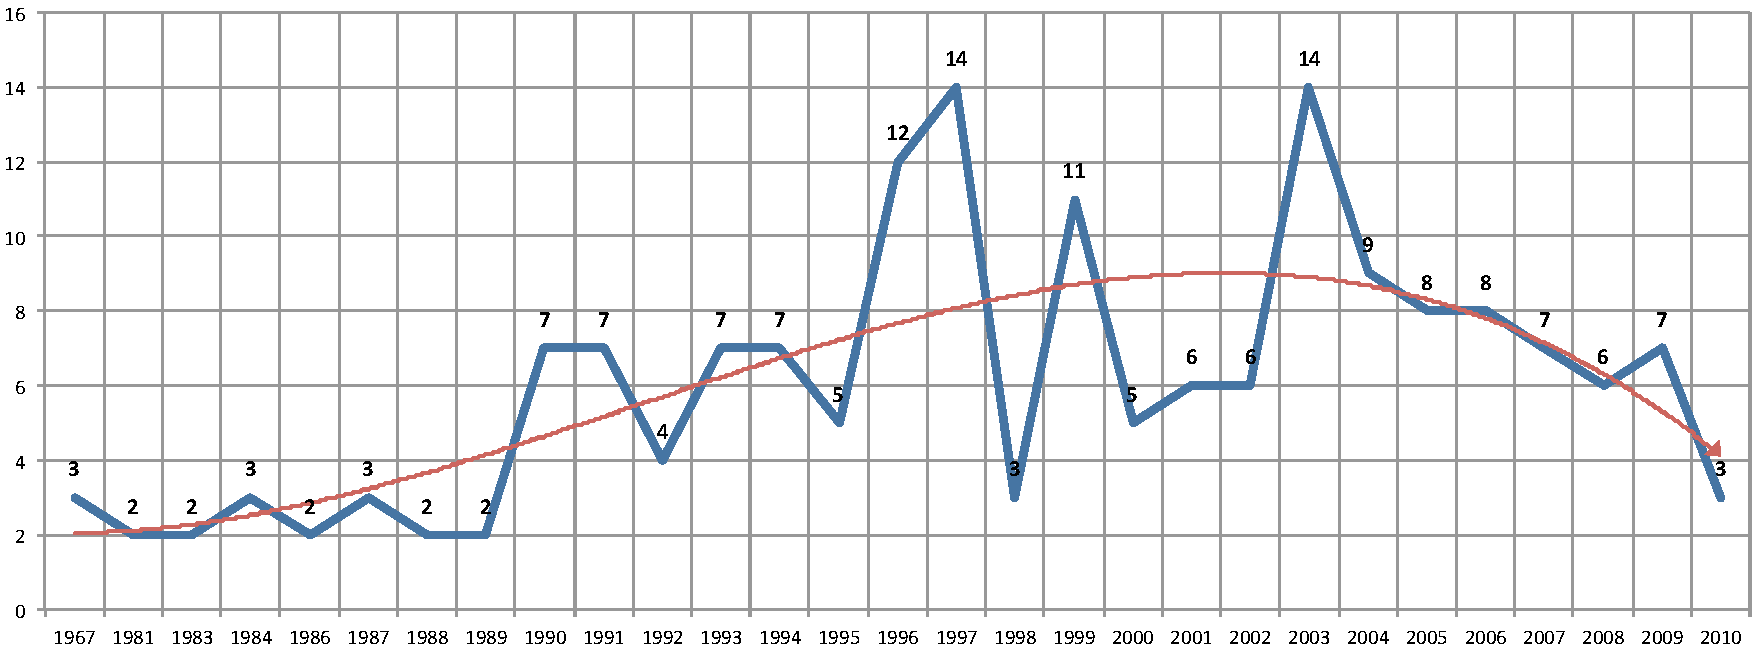
\includegraphics[scale=0.5]{ape_comandos/abntex2-modelo-img-grafico.pdf}
	\end{center}
	\caption{\label{fig_grafico}Gráfico produzido em Excel e salvo como PDF}
	\legend{Fonte: \citeonline[p. 24]{araujo2012}}
\end{figure}

% ---
\section{Enumerações: alíneas e subalíneas}
% ---

\index{alíneas}\index{subalíneas}\index{incisos}Quando for necessário enumerar
os diversos assuntos de uma seção que não possua título, esta deve ser
subdividida em alíneas \cite[4.2]{NBR6024:2012}:

\begin{alineas}

  \item os diversos assuntos que não possuam título próprio, dentro de uma mesma
  seção, devem ser subdivididos em alíneas\footnote{As notas devem ser digitadas ou datilografadas
  dentro das margens, ficando separadas do texto por um espaço simples de entre as
  linhas e por filete de 5 cm, a partir da margem esquerda. Devem ser
  alinhadas, a partir da segunda linha da mesma nota, abaixo da primeira letra
  da primeira palavra, de forma a destacar o expoente, sem espaço entre elas e
  com fonte menor. \citeonline[5.2.1]{NBR14724:2011}}; 
  
  \item o texto que antecede as alíneas termina em dois pontos;
  \item as alíneas devem ser indicadas alfabeticamente, em letra minúscula,
  seguida de parêntese. Utilizam-se letras dobradas, quando esgotadas as
  letras do alfabeto;

  \item as letras indicativas das alíneas devem apresentar recuo em relação à
  margem esquerda;

  \item o texto da alínea deve começar por letra minúscula e terminar em
  ponto-e-vírgula, exceto a última alínea que termina em ponto final;

  \item o texto da alínea deve terminar em dois pontos, se houver subalínea;

  \item a segunda e as seguintes linhas do texto da alínea começa sob a
  primeira letra do texto da própria alínea;
  
  \item subalíneas \cite[4.3]{NBR6024:2012} devem ser conforme as alíneas a
  seguir:

  \begin{alineas}
     \item as subalíneas devem começar por travessão seguido de espaço;

     \item as subalíneas devem apresentar recuo em relação à alínea;

     \item o texto da subalínea deve começar por letra minúscula e terminar em
     ponto-e-vírgula. A última subalínea deve terminar em ponto final, se não
     houver alínea subsequente;

     \item a segunda e as seguintes linhas do texto da subalínea começam sob a
     primeira letra do texto da própria subalínea.
  \end{alineas}
  
  \item no \abnTeX\ estão disponíveis os ambientes \texttt{incisos} e
  \texttt{subalineas}, que em suma são o mesmo que se criar outro nível de
  \texttt{alineas}, como nos exemplos à seguir:
  
  \begin{incisos}
    \item \textit{Um novo inciso em itálico};
  \end{incisos}
  
  \item Alínea em \textbf{negrito}:
  
  \begin{subalineas}
    \item \textit{Uma subalínea em itálico};
    \item \underline{\textit{Uma subalínea em itálico e sublinhado}}; 
  \end{subalineas}
  
  \item Última alínea com \emph{ênfase}.
  
\end{alineas}


% ---
\section{Inclução de outros arquivos}\label{sec-include}
% ---

É uma boa prática dividir o seu documento em diversos arquivos, e não
apenas escrever tudo em um único. Esse recurso foi utilizado neste
documento. Para incluir diferentes arquivos em um arquivo principal,
de modo que cada arquivo incluído fique em uma página diferente, utilize o
comando:

\begin{verbatim}
   \include{documento-a-ser-incluido}      % sem a extensão .tex
\end{verbatim}

Para incluir documentos sem quebra de páginas, utilize:

\begin{verbatim}
   \input{documento-a-ser-incluido}      % sem a extensão .tex
\end{verbatim}

% ---
\section{Compilar o documento \LaTeX}
% ---

Geralmente os editores \LaTeX, como o
TeXlipse\footnote{\url{http://texlipse.sourceforge.net/}}, o
Texmaker\footnote{\url{http://www.xm1math.net/texmaker/}}, entre outros,
compilam os documentos automaticamente, de modo que você não precisa se
preocupar com isso.

No entanto, você pode compilar os documentos \LaTeX usando os seguintes
comandos, que devem ser digitados no \emph{Prompt de Comandos} do Windows ou no
\emph{Terminal} do Mac ou do Linux:

\begin{verbatim}
   pdflatex ARQUIVO_PRINCIPAL.tex
   bibtex ARQUIVO_PRINCIPAL.aux
   makeindex ARQUIVO_PRINCIPAL.idx 
   makeindex ARQUIVO_PRINCIPAL.nlo -s nomencl.ist -o ARQUIVO_PRINCIPAL.nls
   pdflatex ARQUIVO_PRINCIPAL.tex
   pdflatex ARQUIVO_PRINCIPAL.tex
\end{verbatim}

% ---
\section{Divisões do documento: seção}\label{sec-divisoes}
% ---

Esta seção testa o uso de divisões de documentos. Isto é uma seção.

\subsection{Divisões do documento: subseção}

Isto é uma subseção.

\subsubsection{Divisões do documento: subsubseção}

Isto é uma subsubseção.

\subsubsection{Divisões do documento: subsubseção}

Isto é outra subsubseção.

\subsection{Divisões do documento: subseção}\label{sec-exemplo-subsec}

Isto é uma subseção.

\subsubsection{Divisões do documento: subsubseção}

Isto é mais uma subsubseção da \autoref{sec-exemplo-subsec}.

% ---
\section{Este é um exemplo de nome de seção longo. Ele deve estar
alinhado à esquerda e a segunda e demais linhas devem iniciar logo abaixo da
primeira palavra da primeira linha}
% ---

Isso atende à norma \citeonline[seções de 5.2.2 a 5.2.4]{NBR14724:2011} 
 e \citeonline[seções de 3.1 a 3.8]{NBR6024:2012}.


% ---
\section{Consulte o manual da classe \textsf{abntex2}}
% ---

Consulte o manual da classe \textsf{abntex2} \cite{abntex2classe} para uma
referência completa das macros e ambientes disponíveis. Além disso, o manual
possui informações adicionais sobre as normas ABNT observadas pelo \abnTeX.

\end{apendicesenv}
% ---

% ----------------------------------------------------------
% Anexos
% ----------------------------------------------------------
% ---
% Inicia os anexos
% ---
\begin{anexosenv}
% Imprime uma página indicando o início dos anexos
\partanexos
% ---
% Incluir Anexo
% ---
\chapter{Morbi ultrices rutrum lorem.}

%o comando lipsum[] comando serve apenas para incluir texto no documento para efeito de visualização do formato.
\lipsum[1-25]
\section{Test}
\lipsum[1-20]


\end{anexosenv}
\end{comment}

\end{document}